\chapter{Design Analysis and Feasibility}
\section{Safety}
Safety here



\section{Center of gravity (Fraser and Rafał)}

Seeing as the RJ100 is originally a commercial aircraft, converting it to a firefighter aircraft would result in a lot of unnecessary weight, 
for example passenger seats, kitchen and cabin bins ect.
This allows the plane to carry more retardant, meaning better performance for this specific application.
However, by removing the excess weight, the center of gravity is shifted and thus will need to be recalculated.
The RJ100 has an acceptable safe range for the center of gravity as a percentage of the mean aerodynamic chord is 28\% to 44\%.
The plane cannot fly safely if the value of the center of gravity along the x-axis of the plane is outwith this range.
The center of gravity also has to remain within this range before, during and after the ejection of retardant.

\subsection{Method of Analysis}
The process of calculating center of gravity is relatively trivial but can be time consuming if done if done by hand,
especially in this case where there are lots of components being removed, greatly altering the mass.
Using MATLAB instead of hand calculations greatly simplifies the process of changing individual values such as the mass, or the position of objects in the plane, to help achieve the safe center of gravity position. \\ 

According to \cite{baker2020engineering} the formula for the x,y and z value of the center of gravity are shown in the equation \ref{eqn:cog_formula}:

\begin{equation}
\begin{split}
  \bar{x} = \frac{\sum{ \bar{x_{i}} m_{i} }}{ \sum{ m_{i}}} \
  \bar{y} = \frac{\sum{ \bar{y_{i}} m_{i} }}{ \sum{ m_{i}}} \
  \bar{z} = \frac{\sum{ \bar{z_{i}} m_{i} }}{ \sum{ m_{i}}} \
\end{split}
\label{eqn:cog_formula}
\end{equation}

The aircraft mass and center of gravity, before excess weight removal, can effectively be represented in equation \ref{eqn:cog_formula} as a particle with known mass and position.
By representing the aircraft in this way, the center of gravity after the removal of unnecessary weight can be calculated.
The mass of the components to be removed are taken as negative, removing them from the original total mass.
This method for calculating the new center of mass position for the x axis of the plane is shown in the equation \ref{eqn:cg_x_example}


\begin{equation}
\begin{split}
  \bar{x}_{plane_{new}} = \frac{ \sum_{i=1}^{n}{m_{i} x_{i}} - \sum_{j=1}^{m}{m_{j} x_{j}}}{ \sum_{i=1}^{n}{m_{i}} - \sum_{j=1}^{m}{m_{j}}} \\
\end{split}
\label{eqn:cg_new_formula_start}
\end{equation}
Where: \\
$n$ = number of items total \\
$m$ = number of items to be removed \\

Substituting:
\begin{equation}
\begin{split}
  \sum_{i=1}^{n}{m_{i} x_{i}} = m_{plane} \bar{x}_{plane} \\
\end{split}
\label{eqn:m_plane_x_plane_formula}
\end{equation}
and:
\begin{equation}
\begin{split}
  \sum_{i=1}^{n}{m_{i}} = m_{plane} \\
\end{split}
\label{eqn:m_plane_formula}
\end{equation}
Into equation \ref{eqn:cg_new_formula_start}:

\begin{equation}
\begin{split}
  \bar{x}_{plane_{new}} = \frac{ m_{plane} x_{plane} - \sum_{j=1}^{m}{m_{j} x_{j}}}{ m_{plane} - \sum_{j=1}^{m}{m_{j}}} \\
\end{split}
\label{eqn:cg_new_formula_end}
\end{equation}

\subsection{Matlab code}
Applying the method above, code was written in MATLAB to to calculate the new cg position through implementing equation \ref{eqn:cg_new_formula_end}, see appendix \ref{appendix:cg_code}. \\  \\
The data for the components to be removed were formatted into an excel file named “aircraftitems.xlsx” and then imported to be represented in the variable “Data”.
This data included each component's mass and it's center of gravity position.
These position's were taken relative to the standard aircraft axis with the origin at the nose of the aircraft.
Importing the data like this makes it easier to tweak values of masses and position of items on the aircraft to find the desired center of gravity position.

\subsection{Consequence of result of code on design decisions}

The position of the tank along the aircraft was tweaked in order to find a result from the MATLAB code that allowed the position of the center of gravity in the x axis was within the safe limits of 28\% to 44\% of the mean aerodynamic chord.
The value of the x position of the center of gravity of the tank was found to be 16m away from the nose of the aircraft.
This position of the tank results in a center of gravity position of the airplane of 44\% of the aerodynamic chord with the tank full of retardant and 28\% when the tank is full. 

\section{Delivery release system and  Tank Pressurisation (Anton and Fraser)}
Delivery system ect... here
\section{Structural Support (Matthew)}

\subsection{Floor structure}

To support the retardant tank in the aircraft selected, we initially tested the option of removing the floor of the aircraft cabin. This would release additional weight for retardant and would allow for free placement of the tank anywhere in the cabin. Through further research, however, it was discovered that the floor section of the cabin provides extra support for the frame which when removed could increase the likelihood of failure in our aircraft. Also, the floor structure is lightweight due to the use of a honeycomb structure cast from a high-density composite material as shown in Figure  (Honeycomb structure in aircraft flooring). Thus, the removal will not reduce the weight significantly enough to remove it and suffer from the reduced structural strength. 

\begin{figure}[!htbp]
\centering
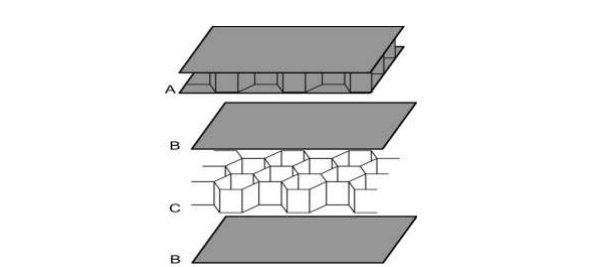
\includegraphics[width= \linewidth]{../figures/honeycomb_structure_in_aircraft_flooring.jpg}
  \caption{Honeycomb structure in aircraft flooring, \cite{ganesh2015design}}
\label{fig:honeycomb_structure_in_aircraft_flooring}
\end{figure}
\FloatBarrier

As the floor panel is to be kept, further structural support for the placement of the tank was considered.  A consideration could be to change the material of the floor beams from aluminum to CFRP (Carbon Fibre Reinforced Plastics), these have a lower weight whilst having higher strength and durability compared to an Aluminum floor. 

\subsection{Beam calculations}
The final length of the tank was estimated using a standard radius of 1.03m which would suitably fit in the aircraft cabin and using a length of 6.55m which resulted in a $15.14 m^3$ volume tank. To support the tank four webs were designed to calculate the resulting stresses and loads, these webs were equally spaced with one at each end as shown in Figure \ref{fig:tank_equal_webs}


\begin{figure}[!htbp]
\centering
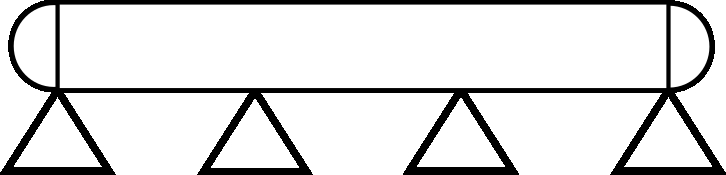
\includegraphics[width= 0.8\linewidth]{../figures/tank_equal_webs.jpg}
\caption{Tank supported by four equally spaced webs}
  \label{fig:tank_equal_webs}
\end{figure}
\FloatBarrier

For the initial calculations the web shape is simplified as shown in figure 3 which will be further refined using FE analysis to gather an accurate final value for the stress distribution. The structure is split into 3 sections as shown and the data representing the sections is displayed in Table (Web structure geometry dimensions).


\begin{figure}[!htbp]
\centering
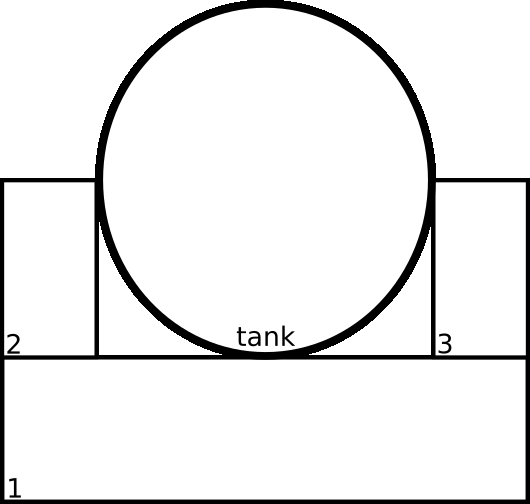
\includegraphics[width= 0.8\linewidth]{../figures/simplified_web_structure.jpg}
\caption{Simplified web structure}
  \label{fig:tank_equal_webs}
\end{figure}
\FloatBarrier

\begin{table}[h!]
  \centering
  \begin{tabular}{|c|c|c|}
    \hline
    Sections & Length(m) & Height (m) \\
    1 & 2.06 & 0.27 \\
    \hline
    2 & 0.2 & 1.17 \\
    \hline
    3 & 9.2 & 1.17 \\
    \hline
  \end{tabular}
  \caption{Web Structure geometry dimensions}
  \label{tab:web_structure_geometry_dimensions}
\end{table}

\subsection{Stress distribution}
The formulae used in these calculations are all standard structural equations as shown to allow for initial estimates: 

\begin{equation}
\begin{split}
  I_{yy} & = \frac{1}{12} d b^{3} + A(\bar{x} - x_{i})^{2} \\ \\
  Z_{e} & = \frac{I_{yy}}{(y_{top} - \bar{y})} \\ \\
  Z_{e_{bottom}} & = \frac{I_{yy}}{(y_{0} - \bar{y})} \\ \\
  R_{y} & = \frac{FL}{4} \\ \\ 
  M_{C/D} & = L R_{y} - \frac{4}{18} FL^{2} \\ \\
  Stress & = \sigma = \frac{M}{Z_{e}} \\ \\
  Load & = \sigma \times Length \times Thickness
\end{split}
  \label{eqn:structures_equations}
\end{equation}

The tank is treated as a uniformly distributed load along the length of the supports and calculations were made at the supports located centrally as these will have the maximum value of stress. The calculations can be seen in appendix \ref{appendix:structural_code}.
\\ \\ 

From these simple calculations a stress distribution plot was produced (Figure \ref{fig:stress_distribution_on_central_supports}) allowing us to analyse the initial feasibility of a four-support system and estimate the total load. 

\begin{figure}[!htbp]
\centering
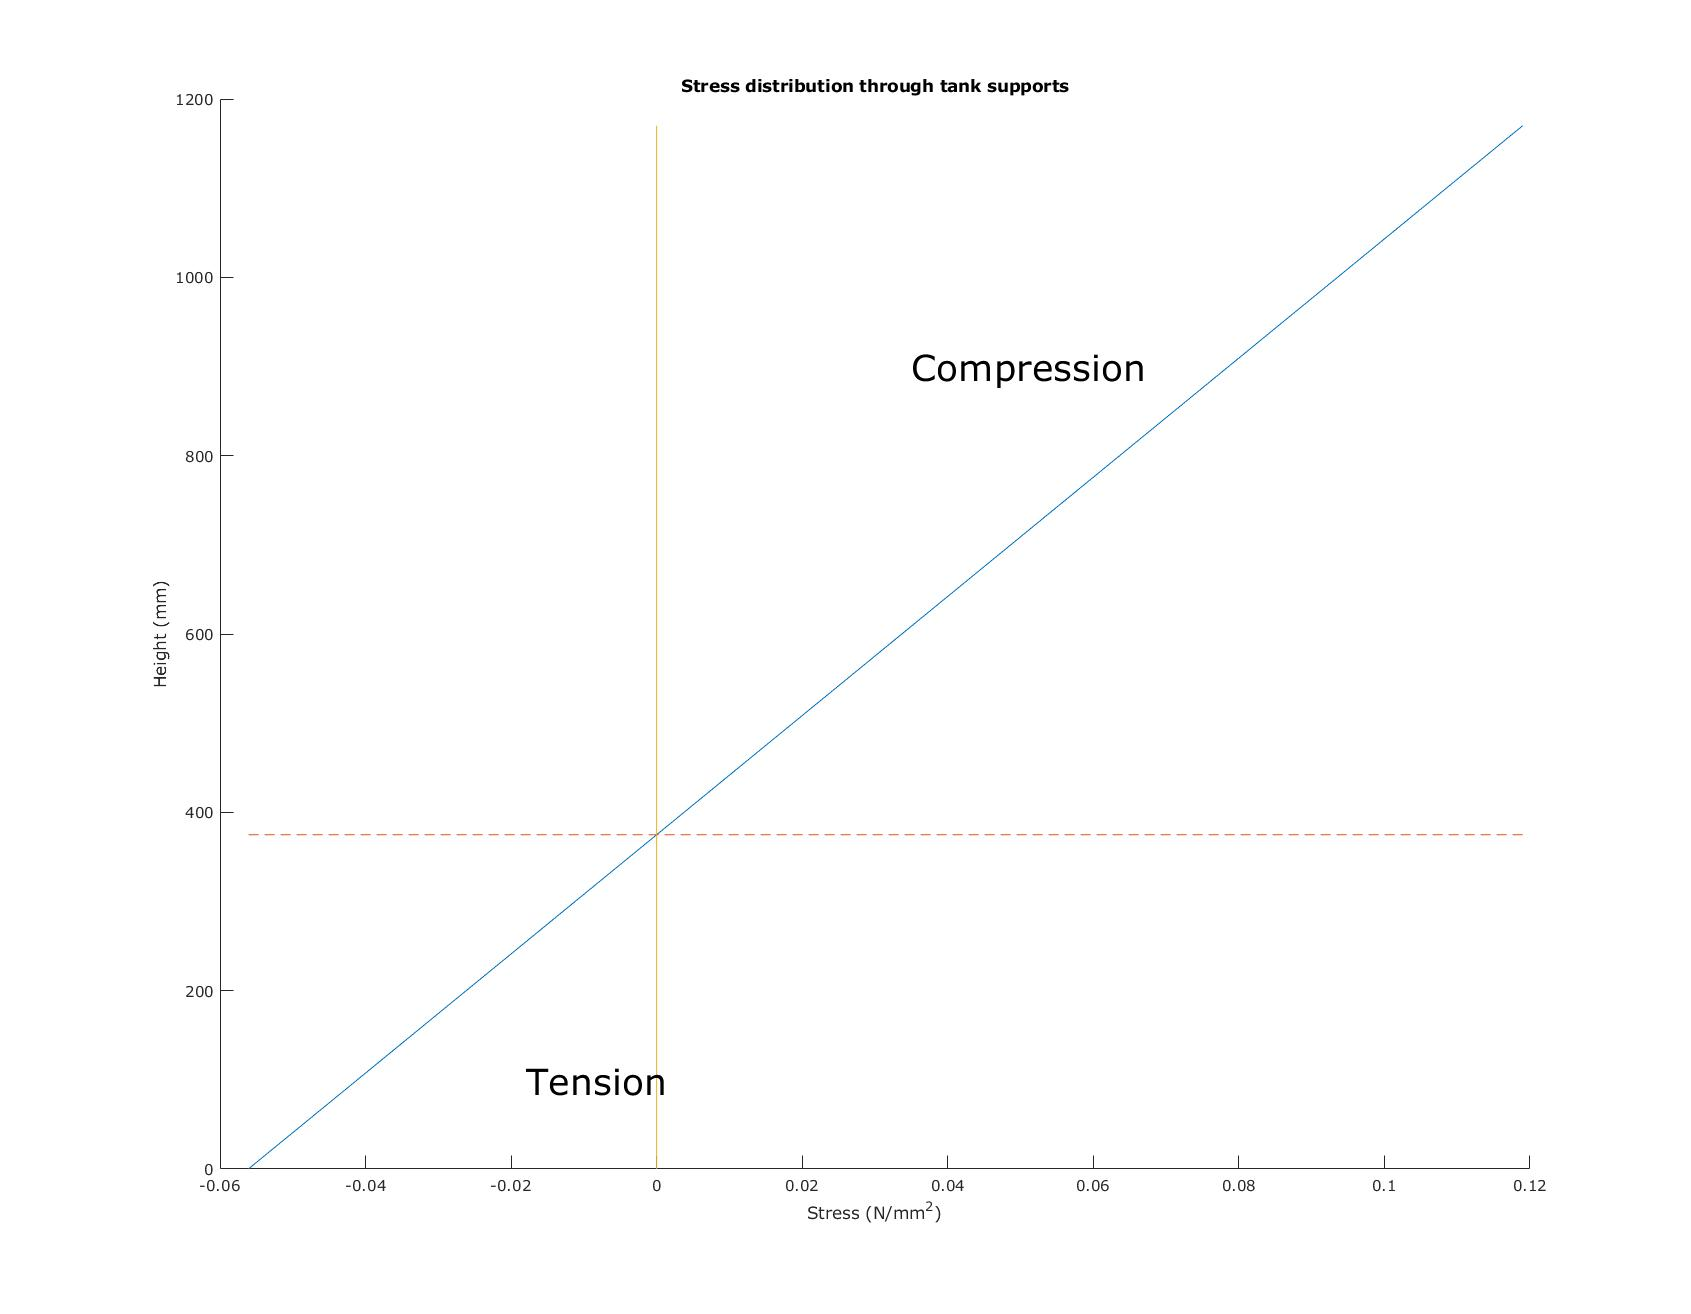
\includegraphics[width= \linewidth]{../figures/stress_distribution_on_central_supports.jpg}
\caption{Stress distribution on central supports}
  \label{fig:stress_distribution_on_central_supports}
\end{figure}
\FloatBarrier

We will need to consider the maximum stress at the bottom of the support to ensure the floor panels in the aircraft have the structural strength to withstand this load. To allow for enough space between the supports the thickness was estimated as $0.1m$ which will add $277.6kg$ to the overall weight of the aircraft reducing the maximum payload achievable slightly. This value of weight is if the material chosen is aluminum with a density of $2710kg/m^3$, chosen as it is regularly used in structural support of aircraft due to its high material strength properties.
Using the stress displayed in figure \ref{fig:stress_distribution_on_central_supports} the total load at the bottom of each support is 18.52kN which will need to be considered when the supports are fixed to the floor.
The maximum stress value is equivalent to $0.12 MPa$ at the top of the structure so the chance of failure is miniscule as shown in the stress-strain curve of aluminium in figure \ref{fig:stress_strain_steel_al}. This value of stress is a considerable distance from failure and even yield so the number of supports could be reduced to save weight in further analysis. 

\begin{figure}[!htbp]
\centering
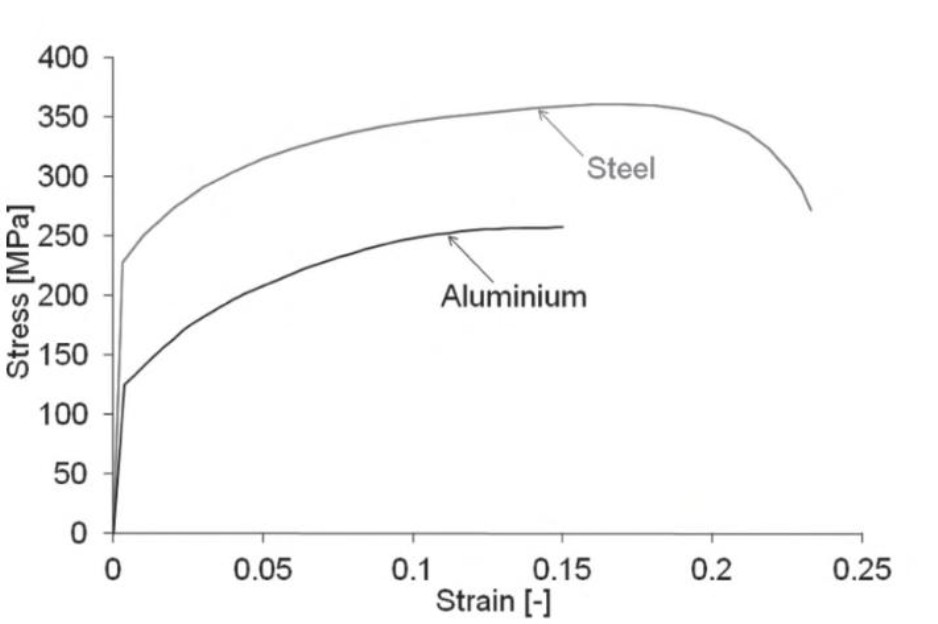
\includegraphics[width= \linewidth]{../figures/stress_strain_steel_al.jpg}
  \caption{Stress-strain curve for steel and aluminum, \cite{liu2013failure}}
  \label{fig:stress_strain_steel_al}
\end{figure}
\FloatBarrier
